\documentclass[border=5pt]{standalone}
\usepackage{tikz}
\usetikzlibrary{shapes.geometric, arrows.meta, positioning, fit, backgrounds, calc}
\usepackage{amsmath}

\newcommand{\Snbr}{S_{\text{nbr}}}

\begin{document}
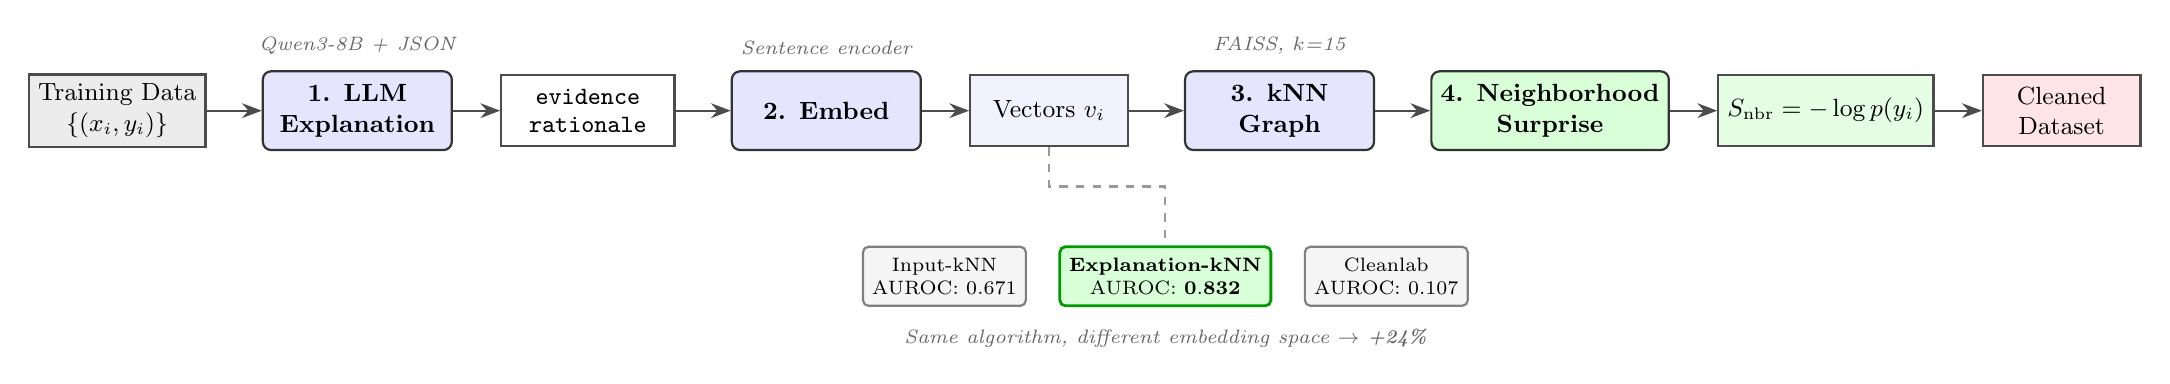
\begin{tikzpicture}[
    node distance=0.4cm and 0.6cm,
    box/.style={rectangle, draw=black!70, fill=white, thick, minimum height=0.9cm, minimum width=2.0cm, align=center, font=\small},
    stage/.style={rectangle, rounded corners=3pt, draw=black!80, fill=blue!10, thick, minimum height=1.0cm, minimum width=2.4cm, align=center, font=\small\bfseries},
    arrow/.style={-{Stealth[length=2.5mm]}, thick, black!70},
    label/.style={font=\scriptsize\itshape, text=black!60},
    compare/.style={rectangle, rounded corners=2pt, draw=black!50, fill=gray!8, thick, minimum height=0.75cm, minimum width=2.0cm, align=center, font=\scriptsize}
]

% Row 1: Full pipeline
\node[box, fill=gray!15] (data) {Training Data\\$\{(x_i, y_i)\}$};

\node[stage, right=0.7cm of data] (explain) {1. LLM\\Explanation};
\node[label, above=0.08cm of explain] {Qwen3-8B + JSON};

\node[box, right=0.6cm of explain, minimum width=2.2cm] (json) {\texttt{evidence}\\[-1pt]\texttt{rationale}};

\node[stage, right=0.7cm of json] (embed) {2. Embed};
\node[label, above=0.08cm of embed] {Sentence encoder};

\node[box, right=0.6cm of embed, fill=blue!5] (vectors) {Vectors $v_i$};

\node[stage, right=0.7cm of vectors] (knn) {3. kNN\\Graph};
\node[label, above=0.08cm of knn] {FAISS, $k$=15};

\node[stage, right=0.7cm of knn, fill=green!15] (surprise) {4. Neighborhood\\Surprise};

\node[box, right=0.6cm of surprise, fill=green!10, minimum width=2.2cm] (score) {$\Snbr = -\log p(y_i)$};

\node[box, right=0.6cm of score, fill=red!10] (output) {Cleaned\\Dataset};

% Arrows - main flow
\draw[arrow] (data) -- (explain);
\draw[arrow] (explain) -- (json);
\draw[arrow] (json) -- (embed);
\draw[arrow] (embed) -- (vectors);
\draw[arrow] (vectors) -- (knn);
\draw[arrow] (knn) -- (surprise);
\draw[arrow] (surprise) -- (score);
\draw[arrow] (score) -- (output);

% Row 2: Comparison boxes centered under pipeline
\node[compare, below=1.2cm of embed, xshift=1.5cm] (input_knn) {Input-kNN\\AUROC: 0.671};
\node[compare, right=0.4cm of input_knn, fill=green!15, draw=green!60!black, line width=1pt] (exp_knn) {\textbf{Explanation-kNN}\\AUROC: $\mathbf{0.832}$};
\node[compare, right=0.4cm of exp_knn] (cleanlab) {Cleanlab\\AUROC: 0.107};

% Annotation
\node[label, below=0.15cm of exp_knn] {Same algorithm, different embedding space $\rightarrow$ \textbf{+24\%}};

% Connection line
\draw[dashed, black!40, thick] (vectors.south) -- ++(0,-0.5) -| (exp_knn.north);

\end{tikzpicture}
\end{document}

